\documentclass[11pt,a4paper]{article}
\usepackage[margin=1in]{geometry}
\usepackage[T1]{fontenc}
\usepackage[utf8]{inputenc}
\usepackage{lmodern}
\usepackage{graphicx}
\usepackage{longtable}
\usepackage{array}
\usepackage{enumitem}
\usepackage{listings}
\usepackage{xcolor}
\usepackage{hyperref}
\lstdefinestyle{pycode}{
  basicstyle=\ttfamily\small,
  backgroundcolor=\color{gray!8},
  frame=single,
  breaklines=true,
  tabsize=4,
  showstringspaces=false,
}
\hypersetup{
  colorlinks=true,
  linkcolor=black,
  urlcolor=blue
}

\title{Dobot Magician Calibration and Setup Guide}
\author{ME403 Introduction to Robotics}
\date{}

\begin{document}
\maketitle

\section{Purpose}
This guide explains the minimum setup required before running Python scripts on a
real Dobot Magician in ME403 labs. The most important prerequisite is
\textbf{calibrating (homing)} with original Dobot software before Python control.

\section{Robot Joint Reference}
The Magician is a 4-axis robot with revolute joints \(J1\) through \(J4\). The
diagram below is useful when interpreting joint commands and measured end-effector
pose in labs.

\begin{center}
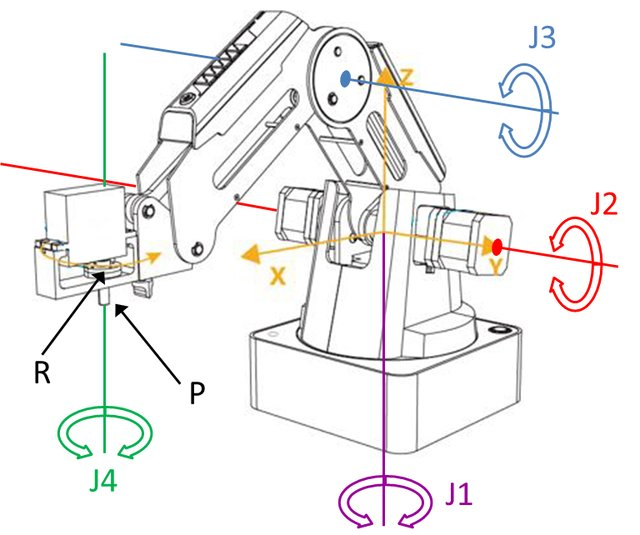
\includegraphics[width=0.88\linewidth]{images/dobot_magician_diagram.jpg}
\end{center}

\subsection*{Joint reminders}
\begin{itemize}[leftmargin=1.5em]
  \item \texttt{J1}: base rotation
  \item \texttt{J2}, \texttt{J3}: arm elevation links (parallelogram structure keeps tool orientation behavior consistent)
  \item \texttt{J4}: end rotation axis
\end{itemize}

\section{Critical Calibration Rule}
\textbf{Always calibrate/home the Magician in original Dobot software before Python runs.}

\begin{itemize}[leftmargin=1.5em]
  \item After power-on, the robot does not reliably know its working reference frame.
  \item Homing re-establishes reference and significantly improves repeatability and parity with simulation.
  \item Dobot software and Python scripts cannot control the same robot at the same time.
\end{itemize}

\section{Download the Original Software}
Use the official Dobot Download Center:

\begin{center}
\url{https://www.dobot-robots.com/service/download-center}
\end{center}

In the \textbf{Control Software} category, download and install
\textbf{DobotStudio (DOBOT Magician) v1.9.4} (released Jan 10, 2022).

\section{Homing Workflow (Recommended)}
\begin{enumerate}[leftmargin=1.5em]
  \item Connect Magician power and USB to your laptop.
  \item Launch DobotStudio.
  \item Click \textbf{Connect} and confirm communication is healthy.
  \item Run \textbf{Home/Calibration} and wait for completion.
  \item In end-effector configuration, select \textbf{None}.
  \item In advanced end-effector options, set XYZ bias to \texttt{0, 0, 0}.
  \item Click \textbf{Disconnect} (or close the application).
  \item Start your Python lab scripts.
\end{enumerate}

\begin{center}
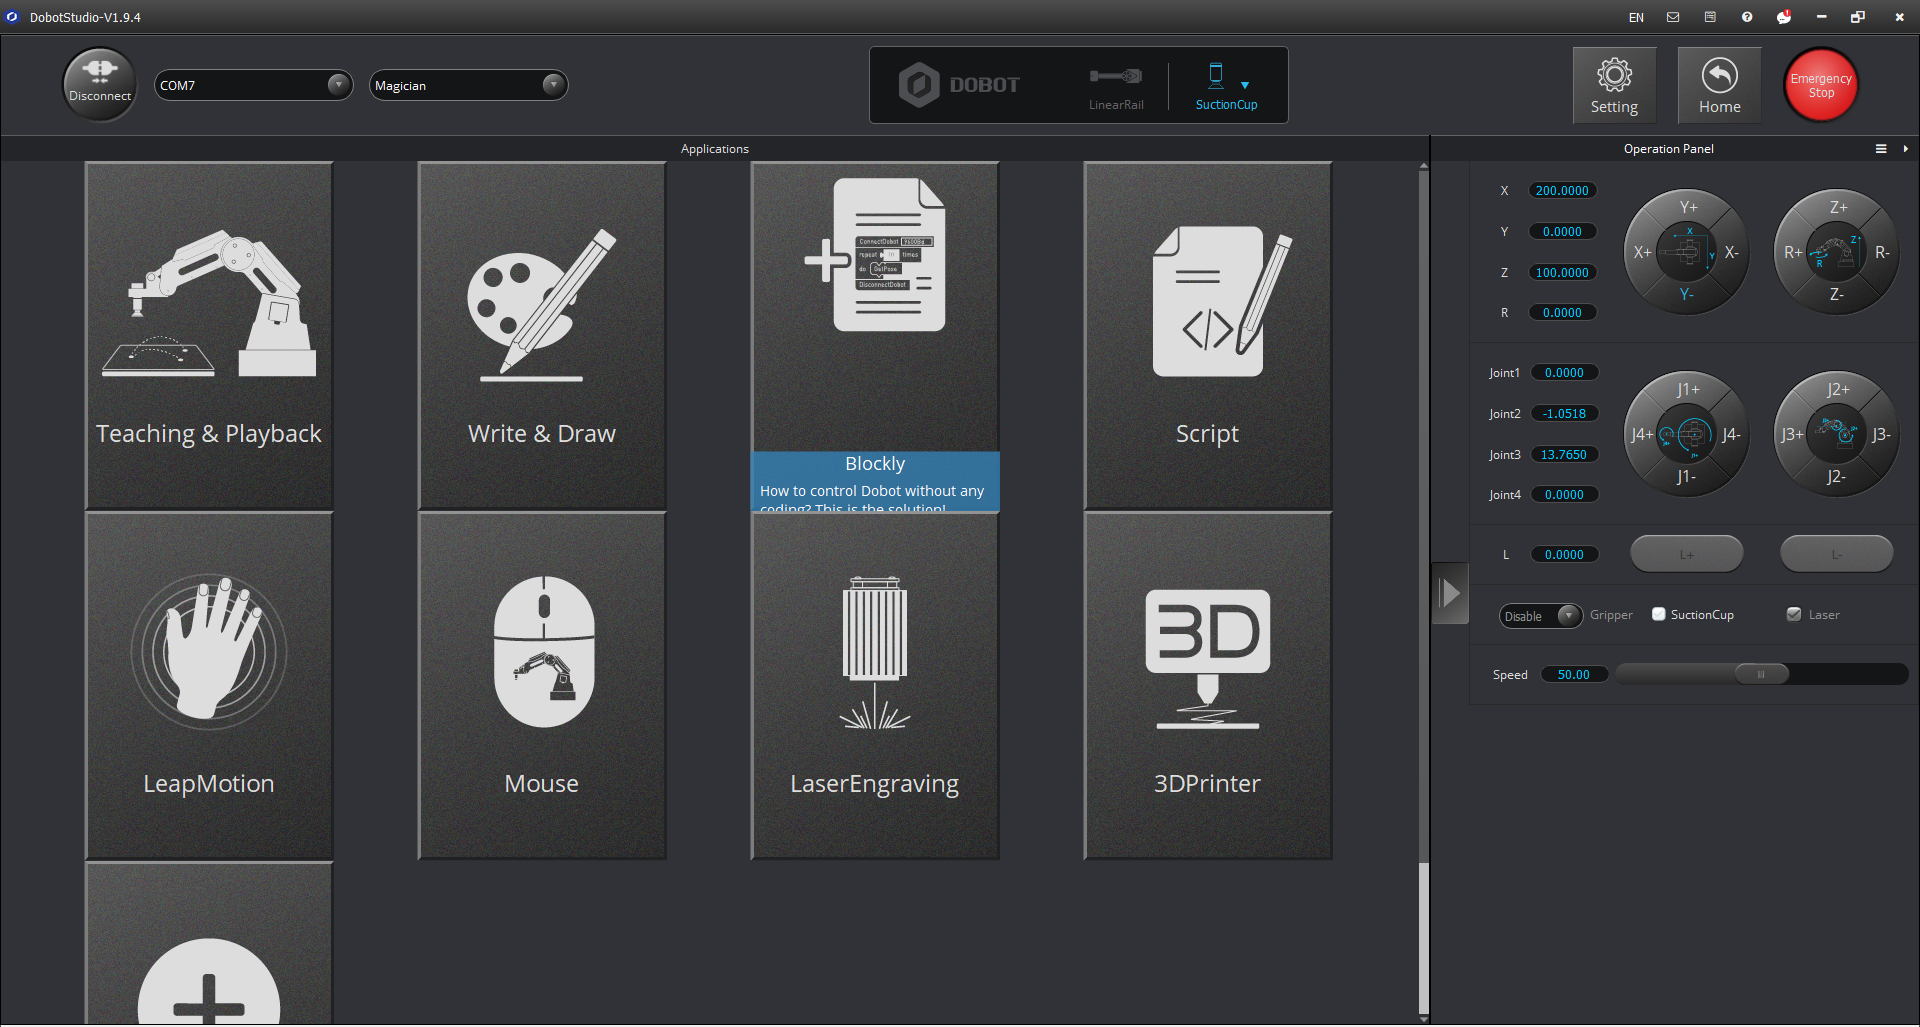
\includegraphics[width=0.96\linewidth]{images/dobotStudio_home.png}
\end{center}

\section{Pre-run Checklist for Python}
\begin{longtable}{|p{0.42\linewidth}|p{0.5\linewidth}|}
\hline
\textbf{Check} & \textbf{Expected state before running Python} \\
\hline
USB + Power & Robot powers on and USB serial device appears \\
\hline
Calibration & Home completed in DobotStudio \\
\hline
Controller ownership & Dobot software disconnected/closed before Python \\
\hline
End-effector config & Type \texttt{None}, advanced XYZ bias \texttt{0,0,0} \\
\hline
Linux permissions & User in \texttt{dialout} group (Linux only) \\
\hline
Sanity probe & \texttt{python3 scripts/check\_magician.py --connect} succeeds \\
\hline
\end{longtable}

\section{Common Failure Modes}
\subsection*{Large real-vs-sim mismatch}
Most commonly caused by skipping calibration/homing before parity or lab runs.
Re-home in Dobot software, disconnect it, then rerun.

\subsection*{Serial device not found}
Check USB/power, close Dobot software, and verify Linux serial permissions.

\subsection*{Robot does not move as expected after long session}
Re-run software homing and restart the Python script to re-initialize state.

\section{Setting End-Effector Type from Python}

Once the robot has been homed in DobotStudio, the TCP offset can be changed
from Python for all subsequent sessions.

\subsection*{Why this matters}

The Magician firmware stores an \((o_x, o_y, o_z)\) bias that shifts every
\texttt{GetPose} result. DobotStudio's ``end-effector type'' selector writes
this bias to the robot's EEPROM via Protocol ID 60.
The same command is available from Python through \texttt{set\_tool\_offset()}
in \texttt{utils.py}.

\subsection*{End-effector preset table}

\begin{center}
\begin{tabular}{|l|l|l|}
\hline
\textbf{Preset} & \textbf{TCP offset (mm)} & \textbf{Home position at (0,0,0,0)} \\
\hline
\texttt{none} (bare flange) & (0,\;0,\;0) & (147,\;0,\;135) mm \\
\hline
\texttt{motor} (motor flange) & (60,\;0,\;0) & (207,\;0,\;135) mm \\
\hline
\texttt{suction} (physical cup tip) & (60,\;0,\;$-$70) & (207,\;0,\;65) mm \\
\hline
\end{tabular}
\end{center}

\textbf{Note on DobotStudio:} The factory ``suction cup'' preset in DobotStudio
uses TCP offset \((+60, 0, 0)\ \mathrm{mm}\) --- same as the motor flange ---
because it reports the motor-shaft TCP, not the physical cup tip. Use the
\texttt{motor} preset (or \texttt{set\_tool\_offset(bot, 60, 0, 0)}) when you
want \texttt{GetPose} to match DobotStudio readings with the suction cup attached.
Use the \texttt{suction} preset to model the physical cup tip for accurate FK/IK.

\subsection*{Python API}

\begin{lstlisting}[style=pycode]
from utils import MAGICIAN_TOOL_OFFSETS, set_tool_offset, get_tool_offset

bot = setup()   # connect to robot

# Read what the firmware currently has
ox, oy, oz = get_tool_offset(bot)
print(f"Current TCP offset: ({ox:.1f}, {oy:.1f}, {oz:.1f}) mm")

# Set to bare flange (required for FK labs)
set_tool_offset(bot, *MAGICIAN_TOOL_OFFSETS["none"])    # writes (0, 0, 0)

# Match DobotStudio "suction cup" factory preset (motor-shaft TCP)
set_tool_offset(bot, *MAGICIAN_TOOL_OFFSETS["motor"])   # writes (60, 0, 0)
\end{lstlisting}

The setting is stored in EEPROM and persists after power-off.

\subsection*{Simulation alignment}

Keep the simulation's \texttt{DOBOT\_EE} environment variable in sync with the
real robot's TCP offset so that FK/IK measurement errors reflect kinematics,
not a mode mismatch:

\begin{verbatim}
# Simulation in bare-flange mode (FK labs default)
DOBOT_EE=none DOBOT_SIMULATION=1 python3 interface.py
\end{verbatim}

\section{ME403 Command Examples}
From \texttt{ME403\_LabFiles/} root:
\begin{verbatim}
python3 scripts/check_magician.py
python3 scripts/check_magician.py --connect
\end{verbatim}

Run Lab 1 interface:
\begin{verbatim}
cd labs/lab01_fk
python3 interface.py
\end{verbatim}

\section{Summary}

\begin{enumerate}[leftmargin=1.5em]
  \item \textbf{Home once} in DobotStudio after power-on.
  \item \textbf{Disconnect} DobotStudio before running Python.
  \item \textbf{Set TCP offset} — either in DobotStudio (type = None) or from
        Python: \texttt{set\_tool\_offset(bot, *MAGICIAN\_TOOL\_OFFSETS["none"])}.
  \item For FK labs, use \textbf{bare-flange mode} (\texttt{none}) on both real
        robot and simulation (\texttt{DOBOT\_EE=none}).
\end{enumerate}

This workflow eliminates the most common setup and parity issues in Magician labs.

\end{document}
